\documentclass[../main.tex]{subfiles}
\begin{document}

\theoremstyle{definition}

\chapter{LU Factorization}

\begin{center}
\textbf{CHAPTER OBJECTIVES}
\end{center}
The primary objective of this chapter is to acquaint you with \textit{LU} factorization.\label{oneLU}\footnote{In the parlance of numerical methods, the terms “factorization” and “decomposition” are synonymous. To be
consistent with the MATLAB documentation, we have chosen to employ the terminology LU factorization for
the subject of this chapter. Note that LU decomposition is very commonly used to describe the same approach.}
Specific objectives and topics covered are
\begin{itemize}
	\item Understanding that \textit{LU} factorization involves decomposing the coefficient matrix into two triangular matrices that can then be used to efficiently evaluate different right-hand-side vectors.
	\item Knowing how to express Gauss elimination as an \textit{LU} factorization.
	\item Given an \textit{LU} factorization, knowing how to evaluate multiple right-hand-side vectors.
	\item Recognizing that Cholesky's method provides an efficient way to decompose a symmetric matrix and that the resulting triangular matrix and its transpose can be used to evaluate right-hand-side vectors efficiently.
	\item Understanding in general terms what happens when MATLAB's backslash operator is used to solve linear systems.
\end{itemize}

As described in Chap. 9, Gauss elimination is designed to solve systems of linear algebraic equations:
$$[A]{x}={b}$$
\begin{flushright}
(10.1)
\end{flushright}
Although it certainly represents a sound way to solve such systems, it becomes inefficient when solving equations with the same coefficients $[A]$, but with different right-hand-side constants $\{b\}$.

Recall that Gauss elimination involves two steps: forward elimination and back substitution (Fig. 9.3). As we learned in Section 9.2.2, the forward-elimination step comprises the bulk of the computational effort. This is particularly true for large systems of equations.

$LU$ factorization methods separate the time-consuming elimination of the matrix $[A]$ from the manipulations of the right-hand side $\{b\}$. Thus, once $[A]$ has been "factored" or "decomposed," multiple right-hand-side vectors can be evaluated in an efficient manner.

Interestingly, Gauss elimination itself can be expressed as an $LU$ factorization. Before showing how this can be done, let us first provide a mathematical overview of the factorization strategy.

\section{OVERVIEW OF LU FACTORIZATION}

Just as was the case with Gauss elimination, $LU$ factorization requires pivoting to avoid division by zero. However, to simplify the following description, we will omit pivoting. In addition, the following explanation is limited to a set of three simultaneous equations. The results can be directly extended to $n$-dimensional systems.

Equation (10.1) can be rearranged to give

\begin{equation}
[A]\{x\}-\{b\}=0\tag{10.2}
\end{equation}
Suppose that Eq. (10.2) could be expressed as an upper triangular system. For example, for a $3 \times 3$ system:
\begin{equation}
\begin{bmatrix}
u_{11} &u_{12}  &u_{13} \\
0 &u_{22}  &u_{23} \\
0 &0  &u_{33}
\end{bmatrix}
\begin{Bmatrix}
x_{1}\\
x_{2}\\
x_{3}
\end{Bmatrix}=
\begin{Bmatrix}
d_{1}\\
d_{2}\\
d_{3}
\end{Bmatrix}\tag{10.3}
\end{equation}
Recognize that this is similar to the manipulation that occurs in the first step of Gauss elimination. That is, elimination is used to reduce the system to upper triangular form. Equation (10.3) can also be expressed in matrix notation and rearranged to give
\begin{equation}
[U]\{x\}-\{d\}=0\tag{10.4}
\end{equation}
Now assume that there is a lower diagonal matrix with 1's on the diagonal,
\begin{equation}
[L]=
\begin{bmatrix}
1 &0  &0 \\
l_{21} &1  &0 \\
l_{31} &l_{32}  &1
\end{bmatrix}\tag{10.5}
\end{equation}
that has the property that when Eq. (10.4) is premultiplied by it, Eq. (10.2) is the result. That is,
\begin{equation}
[L]\{[U]\{x\}-\{d\}\}=[A]\{x\}-\{b\}\tag{10.6}
\end{equation}
If this equation holds, it follows from the rules for matrix multiplication that
\begin{equation}
[L][U]=[A]\tag{10.7}
\end{equation}
and
\begin{equation}
[L]\{d\}=\{b\}\tag{10.8}
\end{equation}

\begin{figure}[H]
	\centering
	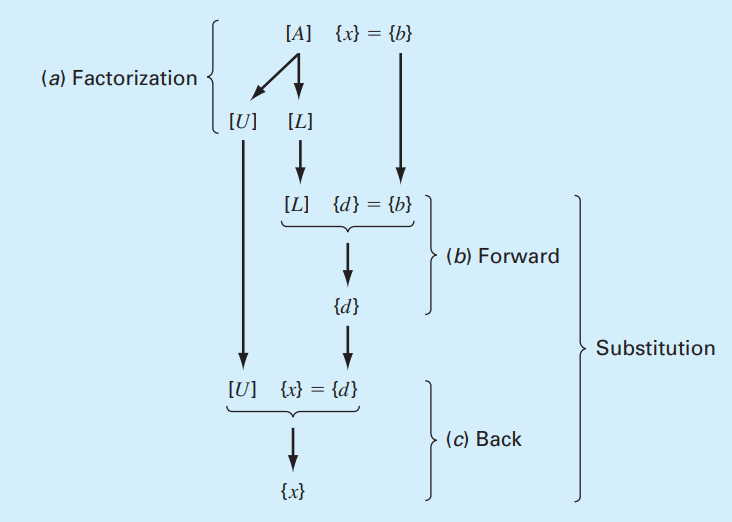
\includegraphics[width=0.75\textwidth]{fig_10_15}
	\caption{\textsf{The steps in LU factorization.}}
	\label{fig:fig_10_15}
\end{figure}

A two-step strategy (see Fig. 10.1) for obtaining solutions can be based on Eqs. (10.3), (10.7), and (10.8):

\begin{enumerate}
\item LU factorization step. [A] is factored or “decomposed” into lower [L] and upper [U] triangular matrices.
\item Substitution step. [L] and [U] are used to determine a solution {x} for a right-hand side $\{b\}$ . This step itself consists of two steps. First, Eq. (10.8) is used to generate an intermediate vector $\{d\}$ by forward substitution. Then, the result is substituted into Eq. (10.3) which can be solved by back substitution for $\{x\}$.
\end{enumerate}
Now let us show how Gauss elimination can be implemented in this way.

\section{GAUSS ELIMINATION AS LU FACTORIZATION}

Although it might appear at face value to be unrelated to LU factorization, Gauss elimination can be used to decompose [A] into [L] and [U]. This can be easily seen for [U], which is a direct product of the forward elimination. Recall that the forward-elimination step is intended to reduce the original coefficient matrix [A] to the form
\begin{equation}
[U]=
\begin{bmatrix}
a_{11} &a_{12}  &a_{13} \\
0 &a'_{22}  &a'_{23} \\
0 &0  &a''_{33}
\end{bmatrix}\tag{10.9}
\end{equation}
which is in the desired upper triangular format.

Though it might not be as apparent, the matrix [L] is also produced during the step. This can be readily illustrated for a three-equation system,
\begin{equation}
\begin{bmatrix}
a_{11} &a_{12}  &a_{13} \\
a_{21} &a_{22}  &a_{23} \\
a_{31} &a_{32}  &a_{33}
\end{bmatrix}
\begin{Bmatrix}
x_{1}\\
x_{2}\\
x_{3}
\end{Bmatrix}=
\begin{Bmatrix}
b_{1}\\
b_{2}\\
b_{3}
\end{Bmatrix}
\end{equation}
The first step in Gauss elimination is to multiply row 1 by the factor [recall Eq. (9.9)]
\begin{equation}
f_{21}=\frac{a_{21}}{a_{11}}
\end{equation}
and subtract the result from the second row to eliminate $a_{21}$. Similarly, row 1 is multiplied by
\begin{equation}
f_{31}=\frac{a_{31}}{a_{11}}
\end{equation}
and the result subtracted from the third row to eliminate $a_{31}$. The final step is to multiply the modified second row by
\begin{equation}
f_{32}=\frac{a'_{32}}{a'_{22}}
\end{equation}
and subtract the result from the third row to eliminate $a'_{32}$.

Now suppose that we merely perform all these manipulations on the matrix [A]. Clearly, if we do not want to change the equations, we also have to do the same to the righthand side $\{b\}$. But there is absolutely no reason that we have to perform the manipulations simultaneously. Thus, we could save the f's and manipulate $\{b\}$ later

Where do we store the factors $f_{21}$, $f_{31}$, and $f_{32}$? Recall that the whole idea behind the elimination was to create zeros in $a_{21}$, $a_{31}$, and $a_{32}$. Thus, we can store $f_{21}$ in $a_{21}$, $f_{31}$ in $a_{31}$, and $f_{32}$ in $a_{32}$. After elimination, the [A] matrix can therefore be written as
\begin{equation}
\begin{bmatrix}
a_{11} &a_{12}  &a_{13} \\
f_{21} &a'_{22}  &a'_{23} \\
f_{31} &f_{32}  &a''_{33}
\end{bmatrix}\tag{10.10}
\end{equation}
This matrix, in fact, represents an efficient storage of the LU factorization of [A],
\begin{equation}
[A]\rightarrow [L][U]\tag{10.11}
\end{equation}
where
\begin{equation}
\begin{bmatrix}
a_{11} &a_{12}  &a_{13} \\
0 &a'_{22}  &a'_{23} \\
0 &0  &a''_{33}
\end{bmatrix}\tag{10.12}
\end{equation}
and
\begin{equation}
\begin{bmatrix}
1 &0  &0 \\
f_{21} &1  &0 \\
f_{31} &f_{32}  &1
\end{bmatrix}\tag{10.13}
\end{equation}
The following example confirms that $[A]=[L][U]$.

\section*{EXAMPLE 10.1 LU Factorization with Gauss Elimination}

Problem Statement. Derive an LU factorization based on the Gauss elimination performed previously in Example 9.3.
Solution. In Example 9.3, we used Gauss elimination to solve a set of linear algebraic equations that had the following coefficient matrix:
\begin{equation}
[A]=\begin{bmatrix}
3 &-0.1  &-0.2 \\
0.1 &7  &-0.3 \\
0.3 &-0.2  & 10
\end{bmatrix}
\end{equation}
After forward elimination, the following upper triangular matrix was obtained:
\begin{equation}
[U]=\begin{bmatrix}
3 &-0.1  &-0.2 \\
0 &7.00333  &-0.293333 \\
0 &0  & 10.0120
\end{bmatrix}
\end{equation}
The factors employed to obtain the upper triangular matrix can be assembled into a lower triangular matrix. The elements a21 and a31 were eliminated by using the factors
\begin{equation}
f_{21}=\frac{0.1}{3}=0.0333333
\; \; \; \; \; \;
f_{31}=\frac{0.3}{3}=0.1000000
\end{equation}
and the element $a_{32}$ was eliminated by using the factor
\begin{equation}
f_{32}=\frac{-0.19}{7.00333}=-0.0271300
\end{equation}
Thus, the lower triangular matrix is
\begin{equation}
[L]=\begin{bmatrix}
1 &0  &0 \\
0.0333333 &1  &0 \\
0.100000 &0.0271300   & 1
\end{bmatrix}
\end{equation}
Consequently, the LU factorization is
\begin{equation}
[A]=[L][U]=\begin{bmatrix}
1 &0  &0 \\
0.0333333 &1  &0 \\
0.100000 &0.0271300   & 1
\end{bmatrix}
\begin{bmatrix}
3 &-0.1  &-0.2 \\
0 &7.00333  &-0.293333 \\
0 &0  & 10.0120
\end{bmatrix}
\end{equation}
This result can be verified by performing the multiplication of [L][U] to give
\begin{equation}
[L][U]=
\begin{bmatrix}
3 &-0.1  &-0.2 \\
0.0999999 &7  &-0.3 \\
0.3 &-0.2  & 9.99996
\end{bmatrix}
\end{equation}
where the minor discrepancies are due to roundoff.

After the matrix is decomposed, a solution can be generated for a particular right-handside vector $\{b\}$. This is done in two steps. First, a forward-substitution step is executed by solving Eq. (10.8) for $\{d\}$. It is important to recognize that this merely amounts to performing the elimination manipulations on $\{b\}$. Thus, at the end of this step, the right-hand side
will be in the same state that it would have been had we performed forward manipulation on [A] and $\{b\}$ simultaneously.

The forward-substitution step can be represented concisely as
\begin{equation}
d_{i}=b_{i}-\sum^{i-1}_{j=1}l_{ij}d_{j}
\; \; \; \; \; \;
for\; \; i=n-1,n-2,\cdots,1
\end{equation}

The second step then merely amounts to implementing back substitution to solve
Eq. (10.3). Again, it is important to recognize that this is identical to the back-substitution phase of conventional Gauss elimination [compare with Eqs. (9.12) and (9.13)]:
\begin{equation}
x_{n}=d_{n}/u_{nn}
\end{equation}
\begin{equation}
x_{i}=\frac{d_{i}-\sum^{n}_{j=i+1}u_{ij}x_{j}}{u{ii}}
\; \; \; \; \; \;
for\; \; i=n-1,n-2,\cdots,1
\end{equation}

\section*{EXAMPLE 10.2 The Substitution Steps}

Problem Statement. Complete the problem initiated in Example 10.1 by generating the
final solution with forward and back substitution.

Solution. As just stated, the intent of forward substitution is to impose the elimination
manipulations that we had formerly applied to $[A]$ on the right-hand-side vector $\{b\}$. Recall that the system being solved is

\begin{equation}
\begin{bmatrix}
3 & -0.1 & -0.2 \\ 
0.1 & 7 & -0.3 \\ 
0.3 & -0.2 & 10
\end{bmatrix}
\begin{Bmatrix}
x_{1}\\ 
x_{2}\\ 
x_{3}
\end{Bmatrix}
=
\begin{Bmatrix}
7.85\\ 
-19.3\\ 
71.4
\end{Bmatrix}
\end{equation}
and that the forward-elimination phase of conventional Gauss elimination resulted in
\begin{equation}
\begin{bmatrix}
3 & -0.1 & -0.2 \\ 
0 & 7.00333 & -0.293333 \\ 
0 & 0 & 10.0120
\end{bmatrix}
\begin{Bmatrix}
x_{1}\\ 
x_{2}\\ 
x_{3}
\end{Bmatrix}
=
\begin{Bmatrix}
7.85\\ 
-19.5617\\ 
70.0843
\end{Bmatrix}
\end{equation}
The forward-substitution phase is implemented by applying Eq. (10.8):
\begin{equation}
\begin{bmatrix}
1 & 0 & 0 \\ 
0.0333333 & 1& 0 \\ 
0.100000 & -0.0271300 & 1
\end{bmatrix}
\begin{Bmatrix}
d_{1}\\ 
d_{2}\\ 
d_{3}
\end{Bmatrix}
=
\begin{Bmatrix}
7.85\\ 
-19.3\\ 
71.4
\end{Bmatrix}
\end{equation}
or multiplying out the left-hand side:
\begin{equation}
d_{1}=7.85\\
0.0333333d_{1}+d_{2}=-19.3\\
0.100000d_{1}-0.0271300d_{2}+d_{3}=71.4
\end{equation}

We can solve the first equation for $d_{1} = 7.85$, which can be substituted into the second equation to solve for
\begin{equation}
d_{2} = -19.3 - 0.0333333(7.85) = -19.5617
\end{equation}
Both $d_{1}$ and $d_{2}$ can be substituted into the third equation to give
\begin{equation}
d_{2} = 71.4 - 0.1(7.85) + 0.02713(-19.5617) = 70.0843
\end{equation}
Thus,
\begin{equation}
\{d\}=
\begin{Bmatrix}
7.85\\
-19.5617\\
70.0843
\end{Bmatrix}
\end{equation}
This result can then be substituted into Eq. (10.3), $[U]\{x\}=\{d\}$:
\begin{equation}
\begin{bmatrix}
3 & -0.1 & -0.2 \\ 
0 & 7.00333 & -0.293333 \\ 
0 & 0 & 10.0120
\end{bmatrix}
\begin{Bmatrix}
x_{1}\\ 
x_{2}\\ 
x_{3}
\end{Bmatrix}
=
\begin{Bmatrix}
7.85\\ 
-19.5617\\ 
70.0843
\end{Bmatrix}
\end{equation}
which can be solved by back substitution (see Example 9.3 for details) for the final solution:
\begin{equation}
\{x\}=
\begin{Bmatrix}
3\\
-2.5\\
7.00003
\end{Bmatrix}
\end{equation}

\section{LU Factorization with Pivoting}
Just as for standard Gauss elimination, partial pivoting is necessary to obtain reliable solutions with LU factorization. One way to do this involves using a permutation matrix (recall Sec. 8.1.2). The approach consists of the following steps:
\begin{enumerate}
\item Elimination. The LU factorization with pivoting of a matrix $[A]$ can be represented in matrix form as
\begin{equation}
[P][A] = [L][U]
\end{equation}
The upper triangular matrix, $[U]$, is generated by elimination with partial pivoting,
while storing the multiplier factors in $[L]$ and employing the permutation matrix, $[P]$, to keep track of the row switches.
\item Forward substitution. The matrices $[L]$ and $[P]$ are used to perform the elimination step with pivoting on $\{b\}$ in order to generate the intermediate right-hand-side vector, $\{d\}$. This step can be represented concisely as the solution of the following matrix
formulation:
\begin{equation}
[L]\{d\} = [P]\{b\}
\end{equation}
\item Back substitution. The final solution is generated in the same fashion as done previously for Gauss elimination. This step can also be represented concisely as the solution of the matrix formulation:
\begin{equation}
[U]\{x\}=\{d\}
\end{equation}
\end{enumerate}
The approach is illustrated in the following example.

\section*{EXAMPLE 10.3 LU Factorization with Pivoting}
Problem Statement. Compute the LU factorization and find the solution for the same
system analyzed in Example 9.4
\begin{equation}
\begin{bmatrix}
0.0003 & 3.0000\\ 
1.0000 & 1.0000
\end{bmatrix}
\begin{Bmatrix}
x_{1}\\ 
x_{2}
\end{Bmatrix}
=
\begin{Bmatrix}
2.0001\\
1.0000
\end{Bmatrix}
\end{equation}
Solution. Before elimination, we set up the initial permutation matrix:
\begin{equation}
[P]=
\begin{bmatrix}
1.0000 & 0.0000\\ 
0.0000 & 1.0000
\end{bmatrix}
\end{equation}
We immediately see that pivoting is necessary, so prior to elimination we switch the rows:
\begin{equation}
[A]=
\begin{bmatrix}
1.0000 & 1.0000\\ 
0.0003 & 3.0000
\end{bmatrix}
\end{equation}
At the same time, we keep track of the pivot by switching the rows of the permutation
matrix:
\begin{equation}
[P]=
\begin{bmatrix}
0.0000 & 1.0000\\ 
1.0000 & 0.0000
\end{bmatrix}
\end{equation}
We then eliminate $a_{21}$ by subtracting the factor $l_{21} = a_{21}/a_{11} = 0.0003/1 = 0.0003$ from the second row of A. In so doing, we compute that the new value of 
$a'_{22} = 3 - 0.0003(1) = 2.9997$. Thus, the elimination step is complete with the result:
\begin{equation}
[U]=
\begin{bmatrix}
1 & 1\\ 
0 & 2.9997
\end{bmatrix}
\end{equation}
\begin{equation}
[L]=
\begin{bmatrix}
1 & 0\\ 
0.0003 & 1
\end{bmatrix}
\end{equation}
Before implementing forward substitution, the permutation matrix is used to reorder
the right-hand-side vector to reflect the pivots as in
\begin{equation}
[P]\{b\}=
\begin{bmatrix}
0.0000 & 1.0000\\ 
1.0000 & 0.0000
\end{bmatrix}
\begin{Bmatrix}
2.0001\\ 
1
\end{Bmatrix}
=
\begin{Bmatrix}
1\\
2.0001
\end{Bmatrix}
\end{equation}
Then, forward substitution is applied as in
\begin{equation}
\begin{bmatrix}
1 & 0\\ 
0.0003 & 1
\end{bmatrix}
\begin{Bmatrix}
d_{1}\\ 
d_{2}
\end{Bmatrix}
=
\begin{Bmatrix}
1\\
2.0001
\end{Bmatrix}
\end{equation}
which can be solved for $d_{1} = 1$ and $d_{2} = 2.0001 - 0.0003(1) = 1.9998$. At this point, the system is
\begin{equation}
\begin{bmatrix}
1 & 1\\ 
0 & 2.9997
\end{bmatrix}
\begin{Bmatrix}
x_{1}\\ 
x_{2}
\end{Bmatrix}
=
\begin{Bmatrix}
1\\
1.9998
\end{Bmatrix}
\end{equation}
Applying back substitution gives the final result:
\begin{equation}
x_{2} = \frac{1.9998}{2.9997} = 0.66667\\
x_{1} = \frac{1 - 1(0.66667)}{1} = 0.33333
\end{equation}
The LU factorization algorithm requires the same total flops as for Gauss elimination.
The only difference is that a little less effort is expended in the factorization phase since the operations are not applied to the right-hand side. Conversely, the substitution phase takes a little more effort.

\subsection{MATLAB Function: lu}

MATLAB has a built-in function lu that generates the LU factorization. It has the general
syntax:

\begin{lstlisting}[numbers=none]
[L,U] = lu(X)
\end{lstlisting}

where L and U are the lower triangular and upper triangular matrices, respectively, derived from the LU factorization of the matrix X. Note that this function uses partial pivoting to avoid division by zero. The following example shows how it can be employed to generate both the factorization and a solution for the same problem that was solved in Examples 10.1 and 10.2.

\section*{EXAMPLE 10.4 LU Factorization with MATLAB}

Problem Statement. Use MATLAB to compute the LU factorization and find the
solution for the same linear system analyzed in Examples 10.1 and 10.2:

\begin{equation}
\begin{bmatrix}
3 & -0.1 & -0.2 \\ 
0.1 & 7 & -0.3 \\ 
0.3 & -0.2 & 10
\end{bmatrix}
\begin{Bmatrix}
x_{1}\\ 
x_{2}\\ 
x_{3}
\end{Bmatrix}
=
\begin{Bmatrix}
7.85\\ 
-19.3\\ 
71.4
\end{Bmatrix}
\end{equation}

Solution. The coefficient matrix and the right-hand-side vector can be entered in standard fashion as

\begin{lstlisting}[numbers=none]
>> A = [3 -.1 -.2;.1 7 -.3;.3 -.2 10];
>> b = [7.85; -19.3; 71.4];
\end{lstlisting}

Next, the LU factorization can be computed with

\begin{lstlisting}[numbers=none]
>> [L,U] = lu(A)
L =
1.0000 0 0
0.0333 1.0000 0
0.1000 -0.0271 1.0000
U =
3.0000 -0.1000 -0.2000
0 7.0033 -0.2933
0 0 10.0120
\end{lstlisting}

This is the same result that we obtained by hand in Example 10.1. We can test that it is correct by computing the original matrix as

\begin{lstlisting}[numbers=none]
>> L*U
ans =
3.0000 -0.1000 -0.2000
0.1000 7.0000 -0.3000
0.3000 -0.2000 10.0000
\end{lstlisting}

To generate the solution, we first compute

\begin{lstlisting}[numbers=none]
>> d = L\b
d =
7.8500
-19.5617
70.0843
\end{lstlisting}

And then use this result to compute the solution

\begin{lstlisting}[numbers=none]
>> x = U\d
x =
3.0000
-2.5000
7.0000
\end{lstlisting}

These results conform to those obtained by hand in Example 10.2

\section{CHOLESKY FACTORIZATION}

Recall from Chap. 8 that a symmetric matrix is one where $a_{ij} = a_{ji}$ for all i and j. In other words, $[A] = [A]^{T}$ . Such systems occur commonly in both mathematical and engineering/science problem contexts.
Special solution techniques are available for such systems. They offer computational
advantages because only half the storage is needed and only half the computation time is
required for their solution.
One of the most popular approaches involves Cholesky factorization (also called
Cholesky decomposition). This algorithm is based on the fact that a symmetric matrix can
be decomposed, as in

\begin{equation}
[A] = [U]^{T} [U]
\tag{10.14}
\end{equation}

That is, the resulting triangular factors are the transpose of each other.
The terms of Eq. (10.14) can be multiplied out and set equal to each other. The factorization can be generated efficiently by recurrence relations. For the ith row:

\begin{equation}
u_{ii}=\sqrt{a_{ii}-\sum_{k=1}^{i-1}u_{ki}^{2}}
\tag{10.15}
\end{equation}

\begin{equation}
u_{ij}=\frac{a_{ij}-\sum_{k=1}^{i-1}u_{ki}u_{kj}}{u_{ii}}
\;\;\; for j=i1,\cdots,n
\tag{10.16}
\end{equation}

\section*{EXAMPLE 10.5 Cholesky Factorization}

Problem Statement. Compute the Cholesky factorization for the symmetric matrix
\begin{equation}
[A]=
\begin{bmatrix}
 6& 15& 55\\ 
15& 55& 225\\ 
55& 225& 979 \\ 
\end{bmatrix}
\end{equation}

Solution. For the first row $(i = 1)$, Eq. (10.15) is employed to compute

\begin{equation}
u_{11} = \sqrt{a_{11}} = \sqrt{6} = 2.44949
\end{equation}
Then, Eq. (10.16) can be used to determine

\begin{equation}
u_{12} = \frac{a_{12}}{u_{11}}
= \frac{15}{2.44949} = 6.123724 \\
u_{13} = \frac{a_{13}}{u_{11}}
= \frac{55}{2.44949} = 22.45366
\end{equation}

For the second row $(i = 2)$:

\begin{equation}
u_{22} = \sqrt{a_{22} - u_{12}^{2}} =
\sqrt{55 - (6.123724)^{2}} = 4.1833\\
u_{23} = \frac{a_{23} - u_{12}u_{13}}{u_{22}} =
= \frac{225 - 6.123724(22.45366)}{4.1833} = 20.9165
\end{equation}

For the third row $(i = 3)$:

\begin{equation}
u_{33} = \sqrt{a_{33} - u_{13}^{2} - u_{23}^{2}} =
\sqrt{979 - (22.45366)^{2} - (20.9165)^{2}} = 6.110101
\end{equation}

Thus, the Cholesky factorization yields

\begin{equation}
[U] =
\begin{bmatrix}
2.44949& 6.123724& 22.45366\\
&4.1833&20.9165\\
&&6.110101
\end{bmatrix}
\end{equation}

The validity of this factorization can be verified by substituting it and its transpose
into Eq. (10.14) to see if their product yields the original matrix [A]. This is left for an exercise.

After obtaining the factorization, it can be used to determine a solution for a righthand-side vector $\{b\}$ in a manner similar to LU factorization. First, an intermediate vector $\{d\}$ is created by solving

\begin{equation}
[U]^{T}\{d\}=\{b\} 
\tag{10.17}
\end{equation}

Then, the final solution can be obtained by solving

\begin{equation}
[U]\{x\}=\{d\} 
\tag{10.17}
\end{equation}

\subsection{MATLAB Function: chol}

MATLAB has a built-in function chol that generates the Cholesky factorization. It has the
general syntax,

\begin{lstlisting}[numbers=none]
U = chol(X)
\end{lstlisting}

where U is an upper triangular matrix so that U'*U = X. The following example shows how
it can be employed to generate both the factorization and a solution for the same matrix that we looked at in the previous example.

\section*{EXAMPLE 10.6 Cholesky Factorization with MATLAB}

Problem Statement. Use MATLAB to compute the Cholesky factorization for the same
matrix we analyzed in Example 10.5.
\begin{equation}
[A] =
\begin{bmatrix}
6& 15& 55\\
15& 55& 225\\
55& 225& 979
\end{bmatrix}
\end{equation}

Also obtain a solution for a right-hand-side vector that is the sum of the rows of [A]. Note that for this case, the answer will be a vector of ones.

Solution. The matrix is entered in standard fashion as

\begin{lstlisting}[numbers=none]
>> A = [6 15 55; 15 55 225; 55 225 979];
\end{lstlisting}

A right-hand-side vector that is the sum of the rows of [A] can be generated as

\begin{lstlisting}[numbers=none]
>> b = [sum(A(1,:)); sum(A(2,:)); sum(A(3,:))]
b =
	76
	295
	1259
\end{lstlisting}

Next, the Cholesky factorization can be computed with

\begin{lstlisting}[numbers=none]
>> U = chol(A)
U =
	2.4495 	6.1237 	22.4537
	0 		4.1833 	20.9165
	0 		0 		6.1101
\end{lstlisting}

We can test that this is correct by computing the original matrix as

\begin{lstlisting}[numbers=none]
>> U'*U
ans =
	6.0000 	15.0000 	55.0000
	15.0000	55.0000 	225.0000
	55.0000	225.0000 	979.0000
\end{lstlisting}

To generate the solution, we first compute

\begin{lstlisting}[numbers=none]
>> d = U'\b
d =
	31.0269
	25.0998
	6.1101
\end{lstlisting}

And then use this result to compute the solution

\begin{lstlisting}[numbers=none]
>> x = U\d
x =
	1.0000
	1.0000
	1.0000
\end{lstlisting}

\section{MATLAB LEFT DIVISION}

We previously introduced left division without any explanation of how it works. Now that
we have some background on matrix solution techniques, we can provide a simplified
description of its operation.

When we implement left division with the backslash operator, MATLAB invokes a
highly sophisticated algorithm to obtain a solution. In essence, MATLAB examines the
structure of the coefficient matrix and then implements an optimal method to obtain the
solution. Although the details of the algorithm are beyond our scope, a simplified overview can be outlined.

First, MATLAB checks to see whether [A] is in a format where a solution can be
obtained without full Gauss elimination. These include systems that are (a) sparse and
banded, (b) triangular (or easily transformed into triangular form), or (c) symmetric. If any of these cases are detected, the solution is obtained with the efficient techniques that are available for such systems. Some of the techniques include banded solvers, back and forward substitution, and Cholesky factorization.

If none of these simplified solutions are possible and the matrix is square,\footnote{It should be noted that in the event that [A] is not square, a least-squares solution is obtained with an approach called QR factorization.} a general
triangular factorization is computed by Gauss elimination with partial pivoting and the
solution obtained with substitution.

\section*{PROBLEMS}

10.1 Determine the total flops as a function of the number
of equations n for the (a) factorization, (b) forward substitution, and (c) back substitution phases of the LU factorization
version of Gauss elimination.


10.2 Use the rules of matrix multiplication to prove that
Eqs. (10.7) and (10.8) follow from Eq. (10.6).


10.3 Use naive Gauss elimination to factor the following
system according to the description in Section 10.2:
\begin{equation}
7x_{1} + 2x_{2} - 3x_{3} = -12\\
2x_{1} + 5x_{2} - 3x_{3} = -20\\
x_{1} - x_{2} - 6x_{3} = -26
\end{equation}
Then, multiply the resulting [L] and [U] matrices to determine that [A] is produced.


10.4 (a) Use LU factorization to solve the system of equations
in Prob. 10.3. Show all the steps in the computation. (b) Also
solve the system for an alternative right-hand-side vector

\begin{equation}
\{b\}^{T} = \left \lfloor 12 \;\;\;\; 18\;\;-6 \right \rfloor
\end{equation}


10.5 Solve the following system of equations using LU
factorization with partial pivoting:
\begin{equation}
2x_{1} - 6x_{2} - x_{3} = -38\\
-3x_{1} - x_{2} + 6x_{3} = -34\\
-8x_{1} + x_{2} - 2x_{3} = -40
\end{equation}


10.6 Develop your own M-file to determine the LU factorization of a square matrix without partial pivoting. That is, develop a function that is passed the square matrix and returns the triangular matrices [L] and [U]. Test your function by
using it to solve the system in Prob. 10.3. Confirm that your
function is working properly by verifying that [L][U] = [A]
and by using the built-in function lu.


10.7 Confirm the validity of the Cholesky factorization of
Example 10.5 by substituting the results into Eq. (10.14) to
verify that the product of $[U]^{T}$ and $[U]$ yields $[A]$.


10.8 (a) Perform a Cholesky factorization of the following symmetric system by hand:
\begin{equation}
\begin{bmatrix}
8& 20& 16\\
20& 80& 50\\
16& 50& 60
\end{bmatrix}
\begin{Bmatrix}
x_{1}\\ 
x_{2}\\ 
x_{3}
\end{Bmatrix}=
\begin{Bmatrix}
100\\ 
250\\ 
100
\end{Bmatrix}
\end{equation}
(b) Verify your hand calculation with the built-in chol
function. (c) Employ the results of the factorization [U] to
determine the solution for the right-hand-side vector.


10.9 Develop your own M-file to determine the Cholesky
factorization of a symmetric matrix without pivoting. That is, develop a function that is passed the symmetric matrix and returns the matrix [U]. Test your function by using it to
solve the system in Prob. 10.8 and use the built-in function chol to confirm that your function is working properly.


10.10 Solve the following set of equations with LU factorization with pivoting:
\begin{equation}
3x_{1} - 2x_{2} + x_{3} = -10\\
2x_{1} + 6x_{2} - 4x_{3} = 44\\
-8x_{1} - 2x_{2} + 5x_{3} = -26
\end{equation}


10.11 (a) Determine the $LU$ factorization without pivoting
by hand for the following matrix and check your results by
validating that $[L][U] = [A]$.
\begin{equation}
\begin{bmatrix}
8& 5& 1\\
3& 7& 4\\
2& 3& 9
\end{bmatrix}
\end{equation}
(b) Employ the result of (a) to compute the determinant. (c) Repeat (a) and (b) using MATLAB.


10.12 Use the following LU factorization to (a) compute
the determinant and (b) solve $[A]\{x\} = \{b\}$ with $\{b\}^{T}=\left \lfloor -10\;\;\;\;50\;\;-26 \right \rfloor$
\begin{equation}
[A] = [L][U] =
\begin{bmatrix}
1&&\\
0.6667& 1&\\
-0.3333& -0.3636& 1
\end{bmatrix}
\times
\begin{bmatrix}
3& -2 & 1\\
&7.3333& -4.6667\\
&&3.6364
\end{bmatrix}
\end{equation}


10.13 Use Cholesky factorization to determine [U] so that
\begin{equation}
[A] = [U]^{T}[U] =
\begin{bmatrix}
2& -1 & 0\\
-1& 2 & -1\\
0& -1 & 2
\end{bmatrix}
\end{equation}


10.14 Compute the Cholesky factorization of 
\begin{equation}
[A] = [U]^{T}[U] =
\begin{bmatrix}
9& 0 & 0\\
0& 25 & 0\\
0& 0 & 16
\end{bmatrix}
\end{equation}

Do your results make sense in terms of Eqs. (10.15) and (10.16)?

\end{document}

